\documentclass[12pt, twoside]{article}
%\documentclass[12pt, twoside]{article}
\usepackage[letterpaper, margin=1in, headsep=0.2in]{geometry}
\setlength{\headheight}{0.6in}
%\usepackage[english]{babel}
\usepackage[utf8]{inputenc}
\usepackage{microtype}
\usepackage{amsmath}
\usepackage{amssymb}
%\usepackage{amsfonts}
\usepackage[nomessages]{fp} %\FPeval{\var-name}{2*sin(pi/6)}
\usepackage{siunitx} %units in math. eg 20\milli\meter
\usepackage{yhmath} % for arcs, overparenth command
\usepackage{tikz} %graphics
\usetikzlibrary{quotes, angles, arrows, arrows.meta}
\usepackage{pgfplots}
\usepgfplotslibrary{fillbetween}
\pgfplotsset{compat=1.16}
\usepackage{graphicx} %consider setting \graphicspath{{images/}}
\usepackage{parskip} %no paragraph indent
\usepackage{enumitem}
\usepackage{multicol}
\usepackage{venndiagram}

\usepackage{fancyhdr}
\pagestyle{fancy}
\fancyhf{}
\renewcommand{\headrulewidth}{0pt} % disable the underline of the header
\raggedbottom
\hfuzz=2mm %suppresses overfull box warnings

\usepackage{hyperref}

\fancyhead[LO]{La Scuola d'Italia / Dr.\ Huson / IB Math 12 (a) \\* 28 October 2026}
\fancyhead[RO]{\fbox{\begin{minipage}{6cm}\footnotesize Nickname:\\[0.5cm]\end{minipage}}}
\fancyhead[LE]{\fbox{\begin{minipage}{6cm}\footnotesize Nickname:\\[0.5cm]\end{minipage}}}
\fancyfoot[C]{\thepage}

\begin{document}
\subsubsection*{2.6 Quiz: Trigonometry}

\begin{center}
\fbox{\begin{minipage}{0.9\textwidth}
\centering
$\dfrac{a}{\sin A} = \dfrac{b}{\sin B} = \dfrac{c}{\sin C}
\qquad
c^{2} = a^{2} + b^{2} - 2ab\cos C
\qquad
\text{Area} = \dfrac{1}{2}ab\sin C$
\end{minipage}}
\end{center}

A calculator is allowed. Give answers correct to three significant figures,
unless they are exact. When a question gives an angle in radians, give
angles in radians. Diagrams are not to scale.

\begin{enumerate}[itemsep=0.15cm]

%--- Problem 1: SAS in radians: cosine rule for a side, area, sine rule for an angle in radians [8 marks] ---
%--- Source: Original (freshly authored, AA SL 3.2, 3.4); parallel of 2-5PQ_Trig-statistics P3 (no unknown x) ---
\item[1.] [Maximum mark: 8]

The following diagram shows triangle $ABC$, with $AB = 6\,\text{cm}$,
$AC = 10\,\text{cm}$ and $B\hat{A}C = 1.1$ radians.

\begin{center}
\begin{tikzpicture}[scale=0.5]
  \coordinate (A) at (0,0);
  \coordinate (B) at (2.722,5.347);
  \coordinate (C) at (10,0);
  \draw[thick] (A) -- (B) -- (C) -- cycle;
  \draw pic["$1.1$", draw, angle radius=0.5cm, angle eccentricity=1.7] {angle = C--A--B};
  \node[below left] at (A) {$A$};
  \node[above] at (B) {$B$};
  \node[below right] at (C) {$C$};
  \node[left] at (1.36,2.67) {$6\,\text{cm}$};
  \node[below] at (5,0) {$10\,\text{cm}$};
\end{tikzpicture}
\end{center}

\begin{enumerate}[itemsep=0.1cm]
  \item Find $BC$. \hfill [3]
  \item Find the area of triangle $ABC$. \hfill [2]
  \item Find $A\hat{C}B$. \hfill [3]
\end{enumerate}

\begin{tikzpicture}
  \draw (-0.6,0) rectangle (14.6,9.5);
  \foreach \y in {1,2,...,8} \draw[dotted] (0,\y)--(14.1,\y);
\end{tikzpicture}

\newpage

%--- Problem 2: Triangular plot (AAS): third angle, sine rule for a side, area; second plot: obtuse angle from area [9 marks] ---
%--- Source: Original (freshly authored, AA SL 3.2); parallel of 2-5PQ_Trig-statistics P4 ---
\item[2.] [Maximum mark: 9]

A triangular plot of land $ABC$ has $AB = 40\,\text{m}$,
$B\hat{A}C = 68^\circ$ and $A\hat{B}C = 47^\circ$.

\begin{center}
\begin{tikzpicture}[scale=0.1]
  \coordinate (A) at (0,0);
  \coordinate (B) at (40,0);
  \coordinate (C) at (12.092,29.928);
  \draw[thick] (A) -- (B) -- (C) -- cycle;
  \draw pic["$68^\circ$", draw, angle radius=0.5cm, angle eccentricity=1.7] {angle = B--A--C};
  \draw pic["$47^\circ$", draw, angle radius=0.5cm, angle eccentricity=1.7] {angle = C--B--A};
  \node[below left] at (A) {$A$};
  \node[below right] at (B) {$B$};
  \node[above] at (C) {$C$};
  \node[below] at (20,0) {$40\,\text{m}$};
\end{tikzpicture}
\end{center}

\begin{enumerate}[itemsep=0.1cm]
  \item Write down $A\hat{C}B$. \hfill [1]
  \item Find $AC$. \hfill [3]
  \item Find the area of the plot. \hfill [2]
\end{enumerate}

A second triangular plot has two sides of length $24\,\text{m}$ and
$35\,\text{m}$. Its area is $320\,\text{m}^{2}$, and the angle between
these two sides is obtuse.

\begin{enumerate}[itemsep=0.1cm]
  \item[(d)] Find the angle between these two sides. \hfill [3]
\end{enumerate}

\begin{tikzpicture}
  \draw (-0.6,0) rectangle (14.6,10.9);
  \foreach \y in {1,2,...,10} \draw[dotted] (0,\y)--(14.1,\y);
\end{tikzpicture}

\newpage

%--- Problem 3: Unit circle: exact coordinates at pi/3, 225 deg in radians and exact coordinates, missing coordinate k, the two solutions of sin(theta) = 0.6 in radians [10 marks] ---
%--- Source: Original (AA SL 3.4, 3.5, 3.8); added 2026-10-28 at Chris's request (replaces the two-boats problem in version (a)) ---
\item[3.] [Maximum mark: 10]

The diagram shows the unit circle, centre $O$. Angles are measured
anticlockwise from the positive $x$-axis. The line $y = 0.6$ meets the
circle at $R$ and $S$.

\begin{center}
\begin{tikzpicture}[scale=2.4]
  \draw[->] (-1.35,0) -- (1.45,0) node[right] {$x$};
  \draw[->] (0,-1.3) -- (0,1.35) node[above] {$y$};
  \draw[thick] (0,0) circle (1);
  \coordinate (O) at (0,0);
  \coordinate (P) at (60:1);
  \coordinate (R) at (36.8699:1);
  \coordinate (S) at (143.1301:1);
  \coordinate (T) at (225:1);
  \draw[dashed] (-1.35,0.6) node[left] {$y = 0.6$} -- (1.35,0.6);
  \draw (O) -- (P);
  \draw (O) -- (R);
  \draw (O) -- (S);
  \draw (O) -- (T);
  \foreach \Q in {P,R,S,T} \fill (\Q) circle (0.5pt);
  \draw (0.25,0) arc (0:60:0.25);
  \node at (47:0.39) {\footnotesize $\frac{\pi}{3}$};
  \draw (0.56,0) arc (0:36.8699:0.56);
  \node at (17:0.66) {\footnotesize $\alpha$};
  \draw (0.82,0) arc (0:143.1301:0.82);
  \node at (98:0.93) {\footnotesize $\beta$};
  \draw (0.13,0) arc (0:225:0.13);
  \node at (205:0.34) {\footnotesize $225^\circ$};
  \node[above right] at (P) {$P(a,\ b)$};
  \node[above right] at (R) {$R(k,\ 0.6)$};
  \node[above left] at (S) {$S$};
  \node[below left] at (T) {$T(c,\ d)$};
  \node[below right] at (0.02,-0.02) {\footnotesize $O$};
  \node[below right] at (1,0) {\footnotesize $1$};
\end{tikzpicture}
\end{center}

\begin{enumerate}[itemsep=0.1cm]
  \item Write down the exact values of $a$ and $b$. \hfill [2]
  \item Write $225^\circ$ in radians, as an exact multiple of $\pi$.
  \hfill [1]
  \item Write down the exact values of $c$ and $d$. \hfill [2]
  \item Find the value of $k$. \hfill [2]
  \item The equation $\sin\theta = 0.6$ has two solutions for
  $0 \leq \theta \leq 2\pi$. They are $\alpha$ and $\beta$. Find $\alpha$
  and $\beta$. \hfill [3]
\end{enumerate}

\begin{tikzpicture}
  \draw (-0.6,0) rectangle (14.6,7.4);
  \foreach \y in {1,2,...,6} \draw[dotted] (0,\y)--(14.1,\y);
\end{tikzpicture}

\newpage

%--- Problem 4: Tree: height from tan, line of sight, angle of elevation from a closer point [7 marks] ---
%--- Source: Original (freshly authored, AA SL 3.3); parallel of 2-5PQ_Trig-statistics P1 ---
\item[4.] [Maximum mark: 7]

A vertical tree $FT$ has its foot $F$ on horizontal ground. Point $A$ is on
the ground, $35\,\text{m}$ from $F$, and the angle of elevation of the top
$T$ from $A$ is $32^\circ$. Point $B$ lies on $[AF]$, $15\,\text{m}$ from
$A$.

\begin{center}
\begin{tikzpicture}[scale=0.12]
  \coordinate (F) at (0,0);
  \coordinate (T) at (0,21.87);
  \coordinate (A) at (-35,0);
  \coordinate (B) at (-20,0);
  \draw[thick] (-40,0) -- (5,0);
  \draw[thick] (F) -- (T);
  \draw (A) -- (T) -- (B);
  \draw pic[draw, angle radius=0.25cm] {right angle = T--F--B};
  \draw pic["$32^\circ$", draw, angle radius=0.7cm, angle eccentricity=1.5] {angle = F--A--T};
  \node[below] at (F) {$F$};
  \node[above] at (T) {$T$};
  \node[below] at (A) {$A$};
  \node[below] at (B) {$B$};
  \node[below] at (-27.5,0) {$15\,\text{m}$};
  \draw[<->] (-35,-6) -- (0,-6) node[midway, below] {$35\,\text{m}$};
\end{tikzpicture}
\end{center}

\begin{enumerate}[itemsep=0.1cm]
  \item Find the height of the tree. \hfill [2]
  \item Find the distance $AT$. \hfill [2]
  \item Find the angle of elevation of $T$ from $B$. \hfill [3]
\end{enumerate}

\begin{tikzpicture}
  \draw (-0.6,0) rectangle (14.6,11.6);
  \foreach \y in {1,2,...,11} \draw[dotted] (0,\y)--(14.1,\y);
\end{tikzpicture}

\end{enumerate}

\newpage

%======================== Version (b) ========================
\fancyhead[LO]{La Scuola d'Italia / Dr.\ Huson / IB Math 12 (b) \\* 28 October 2026}
\subsubsection*{2.6 Quiz: Trigonometry}

\begin{center}
\fbox{\begin{minipage}{0.9\textwidth}
\centering
$\dfrac{a}{\sin A} = \dfrac{b}{\sin B} = \dfrac{c}{\sin C}
\qquad
c^{2} = a^{2} + b^{2} - 2ab\cos C
\qquad
\text{Area} = \dfrac{1}{2}ab\sin C$
\end{minipage}}
\end{center}

A calculator is allowed. Give answers correct to three significant figures,
unless they are exact. When a question gives an angle in radians, give
angles in radians. Diagrams are not to scale.

\begin{enumerate}[itemsep=0.15cm]

%--- Problem 1: Tower seen from two points 50 m apart (no horizontal distance to the foot): show angle ATB, sine rule for BT, height, distance BF [8 marks] ---
%--- Source: Original (freshly authored, AA SL 3.2, 3.3); harder parallel of 2-6Q version (a) P1 ---
\item[1.] [Maximum mark: 8]

Points $A$ and $B$ lie on horizontal ground, in a straight line with the
foot $F$ of a vertical tower $FT$, with $B$ between $A$ and $F$.
$AB = 50\,\text{m}$. The angle of elevation of the top $T$ from $A$ is
$23^\circ$, and from $B$ it is $40^\circ$.

\begin{center}
\begin{tikzpicture}[scale=0.075]
  \coordinate (F) at (0,0);
  \coordinate (T) at (0,42.95);
  \coordinate (B) at (-51.19,0);
  \coordinate (A) at (-101.19,0);
  \draw[thick] (-106,0) -- (6,0);
  \draw[thick] (F) -- (T);
  \draw (A) -- (T) -- (B);
  \draw pic[draw, angle radius=0.25cm] {right angle = T--F--B};
  \draw pic["$23^\circ$", draw, angle radius=0.9cm, angle eccentricity=1.4] {angle = F--A--T};
  \draw pic["$40^\circ$", draw, angle radius=0.6cm, angle eccentricity=1.6] {angle = F--B--T};
  \node[below] at (F) {$F$};
  \node[above] at (T) {$T$};
  \node[below] at (A) {$A$};
  \node[below] at (B) {$B$};
  \node[below] at (-76.19,0) {$50\,\text{m}$};
\end{tikzpicture}
\end{center}

\begin{enumerate}[itemsep=0.1cm]
  \item Show that $A\hat{T}B = 17^\circ$. \hfill [1]
  \item Find $BT$. \hfill [3]
  \item Find the height of the tower. \hfill [2]
  \item Find the distance $BF$. \hfill [2]
\end{enumerate}

\begin{tikzpicture}
  \draw (-0.6,0) rectangle (14.6,7.5);
  \foreach \y in {1,2,...,6} \draw[dotted] (0,\y)--(14.1,\y);
\end{tikzpicture}

\newpage

%--- Problem 2: Ambiguous case in radians: two values of angle PRQ, then the obtuse case: third angle, PR, area [8 marks] ---
%--- Source: Original (freshly authored, AA SL 3.2, 3.4); harder parallel of 2-6Q version (a) P3; cf. 2-4PQ_Mixed-trig P4 ---
\item[2.] [Maximum mark: 8]

In triangle $PQR$, $PQ = 12\,\text{cm}$, $QR = 9\,\text{cm}$ and
$Q\hat{P}R = 0.7$ radians.

\begin{enumerate}[itemsep=0.1cm]
  \item Find the two possible values of $P\hat{R}Q$. \hfill [3]
\end{enumerate}

In the rest of this question, $P\hat{R}Q$ is obtuse.

\begin{enumerate}[itemsep=0.1cm]
  \item[(b)] Find $P\hat{Q}R$. \hfill [1]
  \item[(c)] Find $PR$. \hfill [2]
  \item[(d)] Find the area of triangle $PQR$. \hfill [2]
\end{enumerate}

\begin{tikzpicture}
  \draw (-0.6,0) rectangle (14.6,15.9);
  \foreach \y in {1,2,...,15} \draw[dotted] (0,\y)--(14.1,\y);
\end{tikzpicture}

\newpage

%--- Problem 3: Quadrilateral ABCD split by diagonal AC: cosine rule for AC (obtuse angle), SSS cosine rule for angle ADC, area of the quadrilateral [9 marks] ---
%--- Source: Original (freshly authored, AA SL 3.2); harder parallel of 2-6Q version (a) P2 ---
\item[3.] [Maximum mark: 9]

The following diagram shows quadrilateral $ABCD$, with $AB = 8\,\text{cm}$,
$BC = 5\,\text{cm}$, $CD = 7\,\text{cm}$, $AD = 12\,\text{cm}$ and
$A\hat{B}C = 125^\circ$.

\begin{center}
\begin{tikzpicture}[scale=0.42]
  \coordinate (A) at (0,0);
  \coordinate (B) at (7.486,-2.821);
  \coordinate (C) at (11.614,0);
  \coordinate (D) at (9.897,6.786);
  \draw[thick] (A) -- (B) -- (C) -- (D) -- cycle;
  \draw[dashed] (A) -- (C);
  \draw pic["$125^\circ$", draw, angle radius=0.45cm, angle eccentricity=2.0] {angle = C--B--A};
  \node[left] at (A) {$A$};
  \node[below] at (B) {$B$};
  \node[right] at (C) {$C$};
  \node[above] at (D) {$D$};
  \node[below left] at (3.74,-1.41) {$8\,\text{cm}$};
  \node[below right] at (9.55,-1.41) {$5\,\text{cm}$};
  \node[right] at (10.76,3.39) {$7\,\text{cm}$};
  \node[above left] at (4.95,3.39) {$12\,\text{cm}$};
\end{tikzpicture}
\end{center}

\begin{enumerate}[itemsep=0.1cm]
  \item Find $AC$. \hfill [3]
  \item Find $A\hat{D}C$. \hfill [3]
  \item Find the area of quadrilateral $ABCD$. \hfill [3]
\end{enumerate}

\begin{tikzpicture}
  \draw (-0.6,0) rectangle (14.6,11.4);
  \foreach \y in {1,2,...,10} \draw[dotted] (0,\y)--(14.1,\y);
\end{tikzpicture}

\newpage

%--- Problem 4: Grouped data with two unknown frequencies from n and the estimated mean; estimated sd; effect of a linear transformation on mean and sd [9 marks] ---
%--- Source: Original (freshly authored, AA SL 4.2, 4.3); review of unit 1 (1-10PQ_Statistics P1, 1-8CW_Standard-deviation) ---
\item[4.] [Maximum mark: 9]

The table shows the times, $t$ minutes, taken by $40$ runners to complete
a race.

\begin{center}
\setlength{\tabcolsep}{3.5pt}\renewcommand{\arraystretch}{1.2}
\begin{tabular}{|l|c|c|c|c|c|}
\hline
Time, $t$ & $10 \le t < 20$ & $20 \le t < 30$ & $30 \le t < 40$ & $40 \le t < 50$ & $50 \le t < 60$ \\
\hline
Number of runners & 6 & $p$ & 12 & $q$ & 3 \\
\hline
\end{tabular}
\end{center}

An estimate of the mean time is $31.25$ minutes.

\begin{enumerate}[itemsep=0.1cm]
  \item Find the value of $p$ and the value of $q$. \hfill [4]
  \item Find an estimate of the standard deviation of the times.
  \hfill [2]
\end{enumerate}

Every runner is given a time penalty of $2$ minutes, and the new times are
then written in seconds.

\begin{enumerate}[itemsep=0.1cm]
  \item[(c)] Find an estimate of the mean and of the standard deviation of
  the new times, in seconds. \hfill [3]
\end{enumerate}

\begin{tikzpicture}
  \draw (-0.6,0) rectangle (14.6,13.5);
  \foreach \y in {1,2,...,12} \draw[dotted] (0,\y)--(14.1,\y);
\end{tikzpicture}

\end{enumerate}
\end{document}
